\subsection[Satz von Ladner]{Satz von Ladner}

\begin{frame}
	Frage : Gibt es $\NP$  Probleme , die nicht \NP -vollständig sind , aber auch nicht in $\P$  liegen
\end{frame}
\begin{frame}{\NP -intermediate}
	\begin{figure} 
		%\centering 
		\caption[NP-Intermediate]{$\NP$-Intermediate} 
		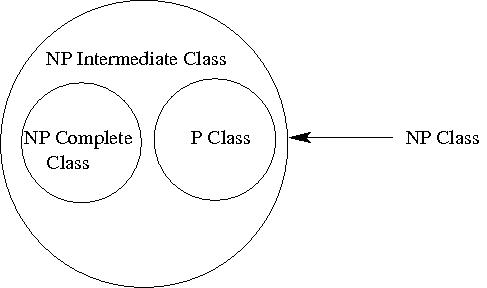
\includegraphics[scale = 0.4]{images/np-intermediate} 
		\newline 
		\label[http://functionspace.org/articles/28/Complexity-Zoo] 
	\end{figure}
\end{frame}
\begin{frame}{\NP -intermediate Probleme}
	Mögliche Kandidaten :
	\begin{itemize}
	\item Graphisomorphie (kommt in Vortrag 7)
	\item Faktorisierungsproblem
	\item Kein "natürlicher" Kandidat bekannt
	\end{itemize}
	
	aber,
\end{frame}

\begin{frame}{Satz von Ladner}
	\begin{Satz}[Existenz einer \NP -intermediate Sprache, Ladner, 75]
	Wenn $\P \neq \NP$ dann gilt : \newline
	Es existiert eine Sprache $L \in \NP \setminus \P$ die nicht \NP -vollständig ist
	\end{Satz}
\end{frame}
\begin{frame}{Beweis von Ladner}
	Wollen eine Sprache konstruieren mit diesen Eigenschaften :
	\pause
	\begin{Definition}[Die Sprache ${\SAT}_H$]
		Für eine Funktion H : $\mathbb{N} \rightarrow \mathbb{N}$ definieren wir : \newline 	
		${\SAT}_H = \lbrace \psi 01^{n^{H(n)}} : \psi \in \SAT$ and $ n = |\psi| \rbrace$
	\end{Definition}

	\pause	
	
	\begin{Beispiel}
	Für $H(n) = n - 1$ und $\psi = a \land b$ gilt : \newline
	$(a \land b) 01^{3^2} = (a \land b) 0111111111 \in {\SAT}_H $
	\end{Beispiel}
	\pause
	${\SAT}_H$ ist also $\SAT$ mit 1er padding
\end{frame}

\begin{frame}{Beweis von Ladner}
	Wir müssen nun also H geschickt wählen !
	\pause
	\begin{block}{Eigenschaft, die wir von H wollen}
		${\SAT}_H \in \P \Leftrightarrow H(n) \in O(1)$ (also $H(n) \leq C$ f\"ur alle n) 				\newline
		und damit insbesondere $\lim_{n \to \infty}  H(n) = \infty$ für ${\SAT}_H \notin \P$
		
	\end{block}	
\end{frame}
\begin{frame}{Nachweis der Eigenschaft von H}
	\begin{Definition}
		H(n) ist die kleinste Gödelnummer $i < \log (\log (n))$ so dass für alle
		$ x \in {0,1}^*$ mit $|x| \leq \log(n) $ die Turing Maschine $M_i$ genau ${\SAT}_H(x)$ 		in $i|x|^i$ Schritten berechnet. Falls dieses i nicht existiert setzen wir $H(n) = 				\log(\log(n))$ 
	\end{Definition}
	\pause
	Zuerst zeigen wir : ${\SAT}_H \in \P \Rightarrow H(n) \in O(1)$
	\pause
	\begin{itemize}[<+->]
		\item ${\SAT}_H \in \P \Rightarrow \exists$ Turing Maschine M, die
			${\SAT}_H$ in höchstens $cn^c$ Schritten entscheidet.
		\item $\exists i > c$ , so dass $M_i$ = M
		\item Für n > $2^{2^i}$ gilt $H(n) \leq i$ und damit $H(n) \in O(1)$ 
	\end{itemize}
\end{frame}